\documentclass[x11names, svgnames]{beamer}
\usepackage[most]{tcolorbox}
\usepackage{tikz}
\usetikzlibrary{shapes.geometric, arrows,chains}
\usetikzlibrary{trees,shapes,snakes}

\definecolor{lightblue}{HTML}{e7f1fa}
\setbeamercolor{block title}{bg=lightblue,fg=black}
\setbeamercolor{block body}{fg=black,bg=gray!20}

\usetheme{sharky}
\usepackage{lipsum}
\usepackage{minibox}
\usepackage{forest}
\usepackage{multicol}

\usepackage[T1]{fontenc}
\usepackage[utf8]{inputenc}
\usepackage{lmodern}
%\setbeamertemplate{blocks}[shadow=true]
\beamertemplatenavigationsymbolsempty
\useinnertheme{circles}

\usepackage[absolute,overlay]{textpos}

\graphicspath{{figures/}}
\setlength{\columnseprule}{0.4pt}

\makeatletter
\newcommand\insertlabelofcurrentframe{%
  \ifx\beamer@againname\@undefined%
  no label%
  \else%
  \beamer@againname%
  \fi%
}
\makeatother

\addtobeamertemplate{headline}{}{%
  \begin{textblock*}{3cm}(0\textwidth,0cm)%
    \tiny \textcolor{gray}{\insertlabelofcurrentframe}%
  \end{textblock*}%
}


\title{\Large{Characterizing the Stability of NISQ Devices}}
\author{\small{Samudra Dasgupta and Travis S. Humble\\Oak Ridge National Laboratory}}
\date{October 16, 2020}

%\author{\small{}}

\begin{document}
\frame[plain]{\titlepage}

\addtocounter{framenumber}{-1}


%%%%%%%%%%%%%%%%%%%%%%%%%%%%%%%%%%%%%%%%%%%%%%%%%%%%%%%%%%%%%
\begin{frame}
\frametitle{Questions we will cover\\\small{Agenda}}
\begin{textblock*}{50mm}(118mm,1mm)
\scriptsize
\textcolor{white}{\textbf{IEEE}}
\end{textblock*}

\scriptsize
Part I:
\begin{itemize}
\item Why the need for a new metric? (Motivating Moment Based Distance)
\item What is the definition of MBD?
\item Is MBD any good vs other methods? (Benchmarking against TVD)
\item How good is the practical approximation? (since the MBD is an infinite series)
\end{itemize}

\vspace{4mm}
Part II:
\begin{itemize}
\item What basic criteria should quantum devices meet to support digital computation? (The DiVincenzo criteria)
\item How should we define the reliabity profile for a Quantum Computer?
\item The concept of temporal stability
\item 
The concept of spatial stability
\end{itemize}
\end{frame}

%%%%%%%%%%%%%%%%%%%%%%%%%%%%%%%%%%%%%%%%%%%%%%%%%%%%%%%%%
\begin{frame}
\frametitle{Part I: What's the need for a new metric?\\\small{Motivating Moment Based Distance}}
\begin{textblock*}{50mm}(118mm,1mm)
\scriptsize
\textcolor{white}{\textbf{IEEE}}
\end{textblock*}

\scriptsize
\begin{itemize}
\item A metric for reproducibility should be simple yet mathematically robust.
\item Contemporary research often use Fidelity and Kullback–Leibler divergence as distribution distance measures. However, neither Fidelity nor Kullback–Leibler divergence satisfy the \textbf{triangle inequality} and hence do not qualify as a \textit{true distance metric}.
\item Another measure commonly in use is the Total Variation Distance (TVD). While it is a true distance metric, it ignores \textbf{higher order effects} (such as kurtosis and skew).
\item Such distance measures could be \textbf{misleading} when used for benchmarking.
\end{itemize}
\end{frame}

\begin{frame}
\frametitle{Part I: What is the definition?\\\small{Moment Based Distance (MBD)}}
\begin{textblock*}{50mm}(118mm,1mm)
\scriptsize
\textcolor{white}{\textbf{IEEE}}
\end{textblock*}

\scriptsize

Given two histograms f and g of a random variable X:\\

\begin{equation}
MBD = d(f,g) = \sum\limits_{m=0}^{\infty} S_m(f, g)
\end{equation}

\begin{equation}
S_{m}(f,g) = \frac{1}{(m)!}\int\limits_a^{b} \left| \left( \frac{x}{\gamma} \right)^{m}(f(x) - g(x))\right|dx
\end{equation}

\begin{equation}
\gamma = \max( |a|,|b|)
\end{equation}

\end{frame}

%%%%%%%%%%%%%%%%%%%%%%%%
\begin{frame}
\frametitle{Part I: Sample case for histogram comparison\\ \small{Please ignore details as we have not covered the concepts yet}}
\begin{textblock*}{50mm}(118mm,1mm)
\scriptsize
\textcolor{white}{\textbf{IEEE}}
\end{textblock*}
\begin{textblock*}{100mm}(5mm,92mm)
\scriptsize
\textcolor{white}{SOURCE: arXiv: 2008.09612}
\end{textblock*}
\vspace{0.1in}

\begin{tabular}{cl}  
\begin{tabular}{c}
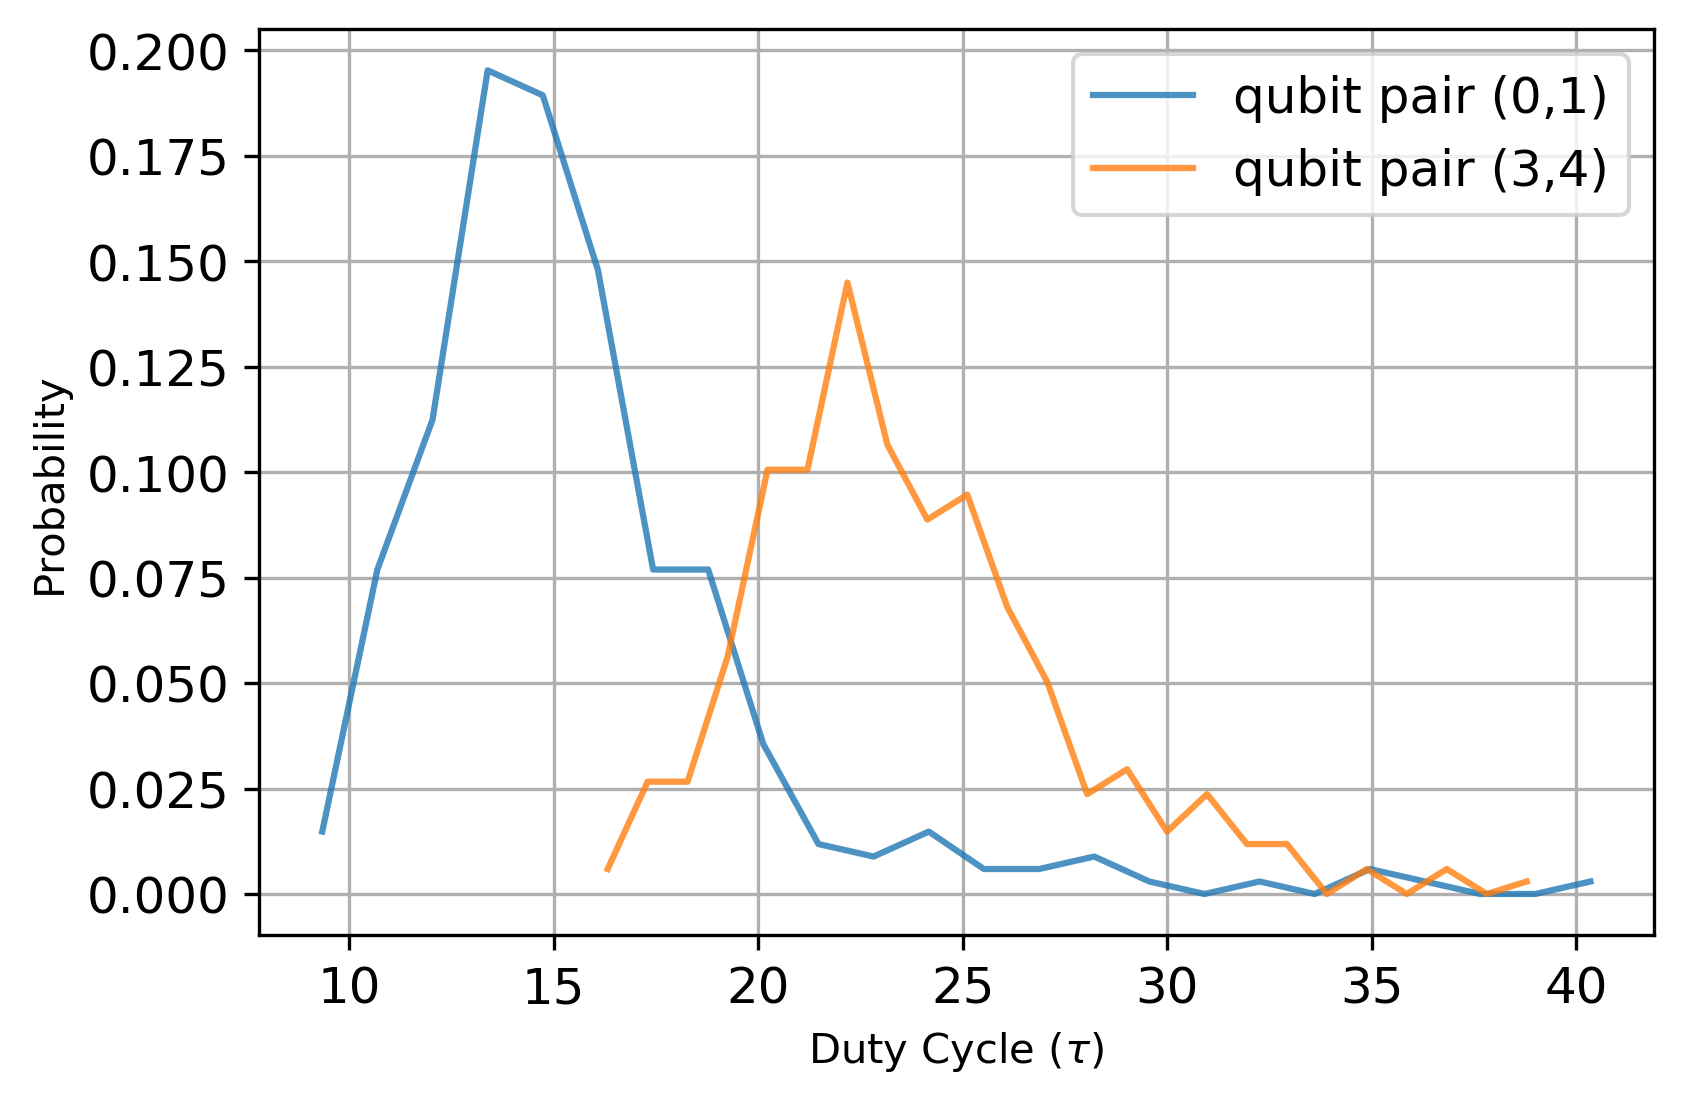
\includegraphics[width=6.6cm]{tau_spatial_twoHists.png}
\end{tabular}
& \begin{tabular}{l}
\scriptsize
\parbox{0.3\linewidth}{


\begin{itemize}
\item Experimental histograms of the duty cycle $\tau$ for qubit pairs that are observed to be furthest (spatially) in the sense of the moment-based distance. The data history spans from March 2019 to March 2020.
\end{itemize}
}
\end{tabular}
\end{tabular}

\end{frame}

%%%%%%%%%%%%%%%%%%%%%%%%%%%

\begin{frame}
\frametitle{Part I: Can we get a feel for the formula?\\ \small{Illustrative example}}
\begin{textblock*}{50mm}(118mm,1mm)
\scriptsize
\textcolor{white}{\textbf{IEEE}}
\end{textblock*}
\begin{textblock*}{100mm}(5mm,92mm)
\scriptsize
\textcolor{white}{SOURCE: arXiv: 2008.09612}
\end{textblock*}
\vspace{0.1in}

\begin{tabular}{cl}  
\begin{tabular}{c}
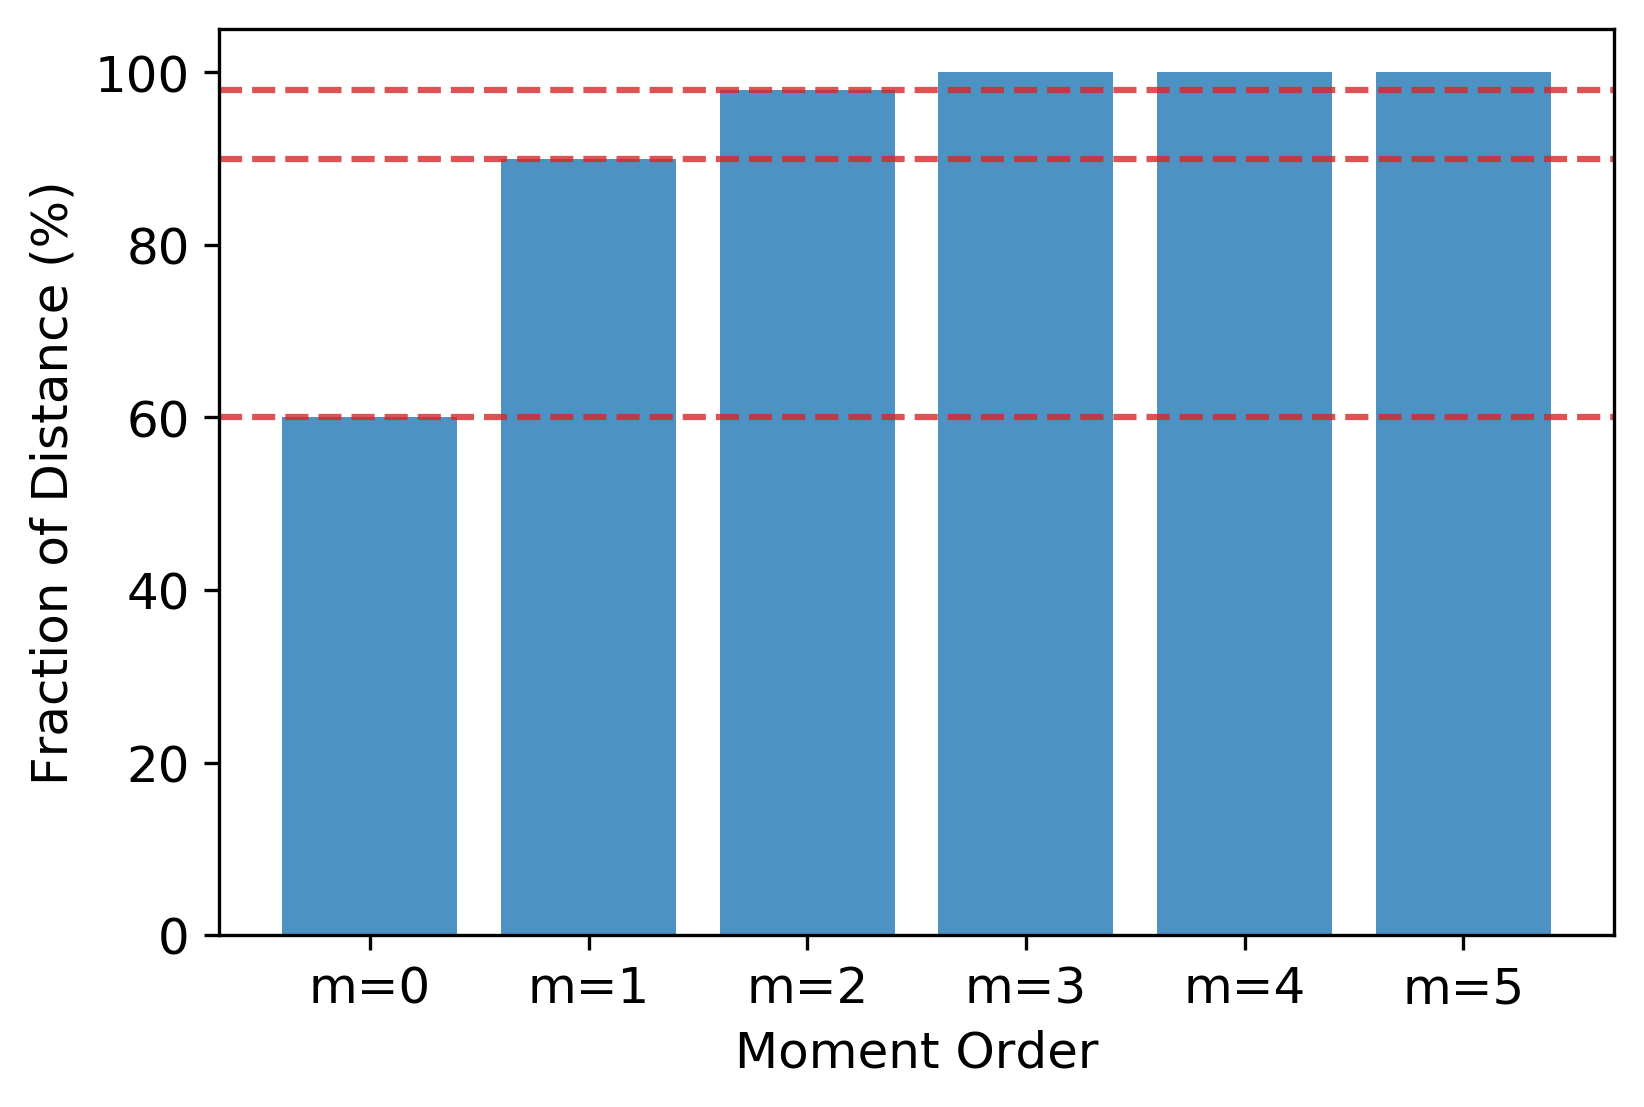
\includegraphics[width=6.6cm]{dnN_unequal_relative.png}
\end{tabular}
& \begin{tabular}{l}
\scriptsize
\parbox{0.3\linewidth}{


\begin{itemize}
\item We compare two normal distributions:
\item $\mathcal{N}_1(\mu_0, \sigma_0)$
\item $\mathcal{N}_2(2\mu_0, 2\sigma_0)$
\item  Plot shows how MBD converges (in other words, how the approximations improve and stabilize quickly.)
\end{itemize}
}
\end{tabular}
\end{tabular}

\begin{center}
\minibox[frame]{Contribution to moment based distance ($d$) from \\increasing moment orders.}
\end{center}
\end{frame}

%%%%%%%%%%%%%%%%%%%%
\begin{frame}
\frametitle{Part I: Is MBD any good vs other methods?\\ \small{Benchmarking against TVD}}
\begin{textblock*}{50mm}(118mm,1mm)
\scriptsize
\textcolor{white}{\textbf{IEEE}}
\end{textblock*}
\begin{textblock*}{100mm}(5mm,92mm)
\scriptsize
\textcolor{white}{SOURCE: arXiv: 2008.09612}
\end{textblock*}
\vspace{0.1in}

\begin{tabular}{cl}  
\begin{tabular}{c}
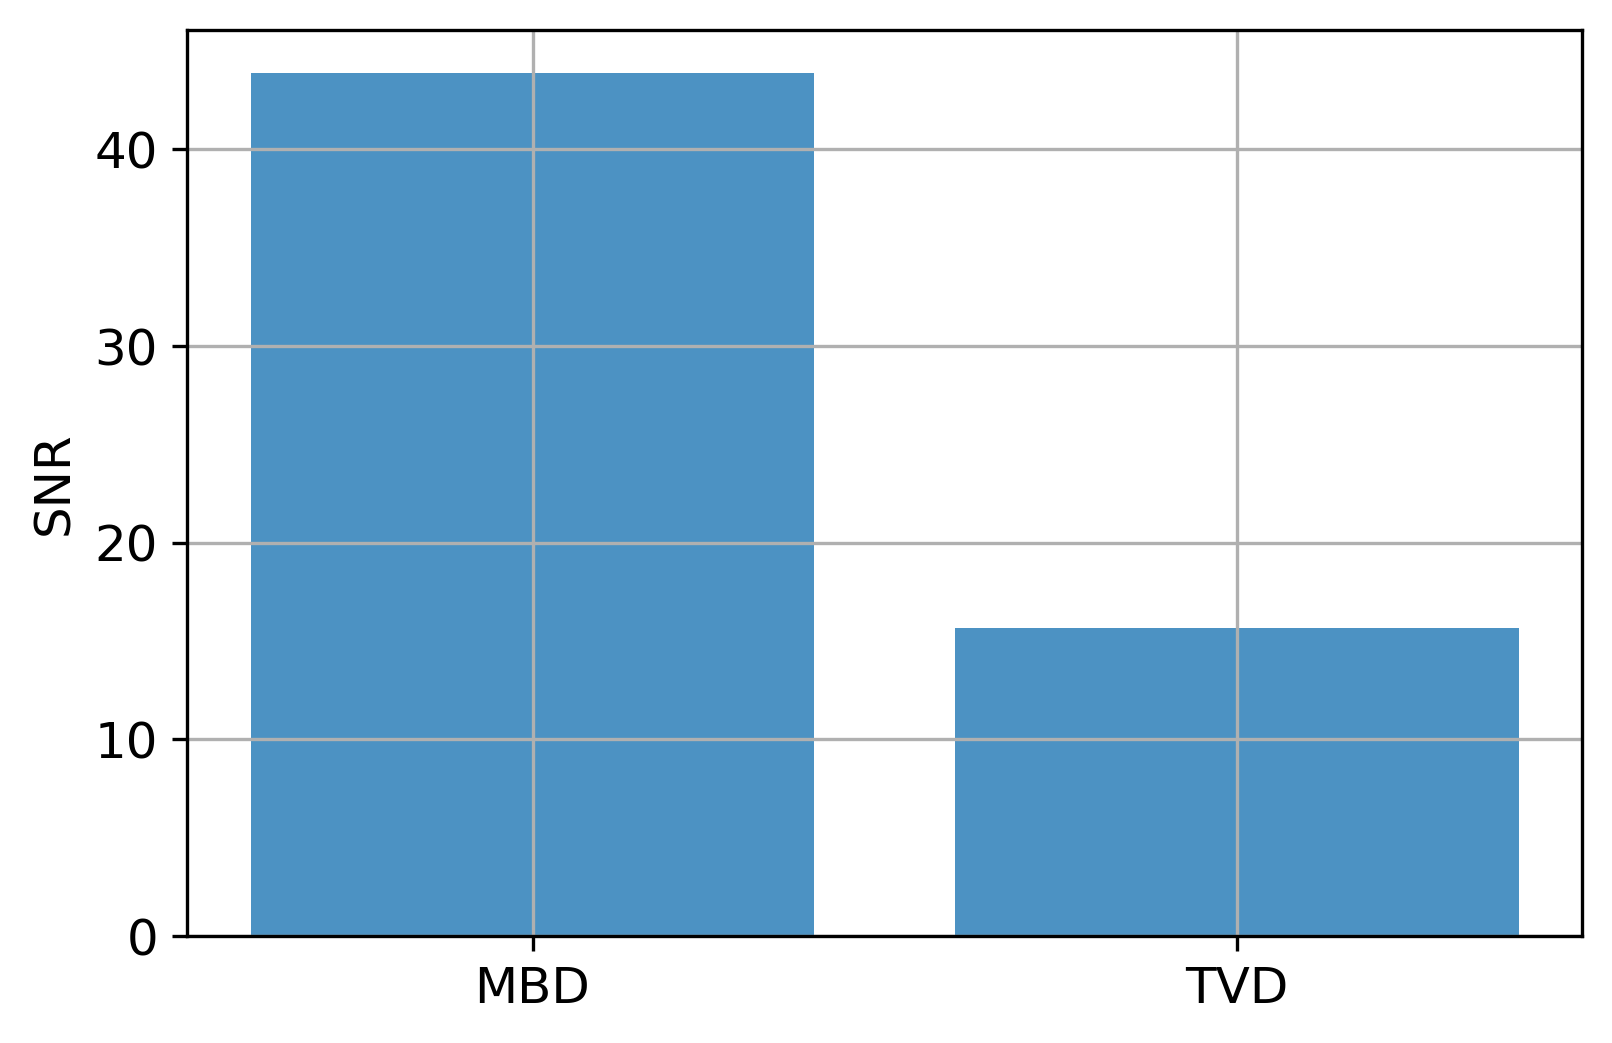
\includegraphics[width=4.4cm]{tvd_d4_info.png}
\end{tabular}
& \begin{tabular}{l}
\scriptsize
\parbox{0.48\linewidth}{

\begin{itemize}
\item Distance metric from different methodologies are not comparable. One can however compare robustness (using SNR). 
\item We generated 2 timeseries, by sampling 2 different distributions, and calculate the MBD and TVD between these timeseries
\item We repeat this 400 times to generate a \textbf{distribution of the TVD and MBD distances}.
\end{itemize}
}
\end{tabular}
\end{tabular}

\begin{center}
\minibox[frame]{\scriptsize
MBD could have more statistical power as indicated by a higher SNR.}
\end{center}
\end{frame}

%%%%%%%%%%%%%%%%%%%%%%%%%%%
\begin{frame}
\frametitle{Part I: How good is the approximation?\\ \small{Remember MBD is an infinite series}}
\begin{textblock*}{50mm}(118mm,1mm)
\scriptsize
\textcolor{white}{\textbf{IEEE}}
\end{textblock*}
\begin{textblock*}{100mm}(5mm,92mm)
\scriptsize
\textcolor{white}{SOURCE: arXiv: 2008.09612}
\end{textblock*}
\vspace{0.1in}

\begin{table}[htbp]
\begin{tabular}{|l|c|c|c|}
\hline
Distribution & $d_4$ & $d_{20}$ & Error(\%)\\
\hline
$N(\mu, \sigma)$ & 0.00000 & 0.00000 & NA\\
\hline
$N(\mu+\Delta, \sigma)$ & 2.70868 & 2.70876 & -0.00289\\
\hline
$N(\mu, 2\sigma)$ & 0.83252 & 0.83253 & -0.00104\\
\hline
$N(\mu, 4\sigma)$ & 1.47301 & 1.47304 & -0.00180\\
\hline
$N(2\mu, \sigma)$ & 2.93489 & 2.93520 & -0.01033\\
\hline
$N(\mu, 1.5\sigma)$ & 0.49215 & 0.49216 & -0.00091\\
\hline
$N(1.01\mu, \sigma)$ & 0.11739 & 0.11740 & -0.00079\\
\hline
$Skewed Normal(\mu, 2\sigma)$ & 0.80887 & 0.80888 & -0.00140\\
\hline
$Gumbel(\mu, 2\sigma)$ & 0.95131 & 0.95134 & -0.00246\\
\hline
\end{tabular}
\end{table}
\end{frame}

%%%%%%%%%%%%%%%%%%%%%%
\begin{frame}
\frametitle{Part II: What basic criteria should quantum \\devices meet to support digital computation?\\ \small{The DiVincenzo criteria}}
\begin{textblock*}{50mm}(118mm,1mm)
\scriptsize
\textcolor{white}{\textbf{IEEE}}
\end{textblock*}
\begin{textblock*}{100mm}(5mm,92mm)
\scriptsize
\textcolor{white}{SOURCE: arXiv: 2008.09612}
\end{textblock*}
\vspace{0.1in}

\begin{itemize}
    \item Host a scalable array of well-defined and addressable quantum physical systems
    \item Support initialization of the quantum state of these physical systems to a well-defined fiducial state
    \item Realize a universal set of gate operations
    \item Maintain the coherence of the quantum state much longer than the duration of any individual gate
    \item Support addressable measurements of each quantum physical system
\end{itemize}

\end{frame}

%%%%%%%%%%%%%%%%%%%%%%
\begin{frame}
\frametitle{Part II: How can we define the\\ reliabity profile for a Quantum Computer?\\ \small{Device metrics using DiVincenzo criteria}}
\begin{textblock*}{50mm}(118mm,1mm)
\scriptsize
\textcolor{white}{\textbf{IEEE}}
\end{textblock*}
\begin{textblock*}{100mm}(5mm,92mm)
\scriptsize
\textcolor{white}{SOURCE: arXiv: 2008.09612}
\end{textblock*}
\vspace{0.1in}

\begin{table}[ht]
    \centering
    \begin{tabular}{|p{4cm}|p{6.4cm}|}
        \hline 
        \textit{Device Metric} (\textit{Symbol}) & \textit{Description} \\ \hline
        Register Capacity ($n$) & The maximal amount of information that may be stored in the register.  \\ \hline
        Initialization Fidelity ($F_{\textrm{I}}$) & The accuracy with which the register state is prepared as the fidelity state. \\ \hline
        Gate Fidelity ($F_{\textrm{G}}$) & The accuracy with which a gate operation prepares the expected output. \\ \hline
        Duty Cycle ($\tau$) & The ratio of the gate duration to coherence time. \\ \hline
        Addressability ($F_{\textrm{A}}$) & The ability to address qubits individually. \\ \hline
    \end{tabular}
\end{table}
\end{frame}

%%%%%%%%%%%%%%%%%%%%%%%%%%%%%%
\begin{frame}
\frametitle{Part II: Let's look at a sample dataset\\ \small{CNOT Gate Fidelity data between 0 and 1 for IBM Yorktown}}
\begin{textblock*}{50mm}(118mm,1mm)
\scriptsize
\textcolor{white}{\textbf{IEEE}}
\end{textblock*}
\begin{textblock*}{100mm}(5mm,92mm)
\scriptsize
\textcolor{white}{SOURCE: arXiv: 2008.09612}
\end{textblock*}
\vspace{0.1in}

\begin{tabular}{cl}  
\begin{tabular}{c}
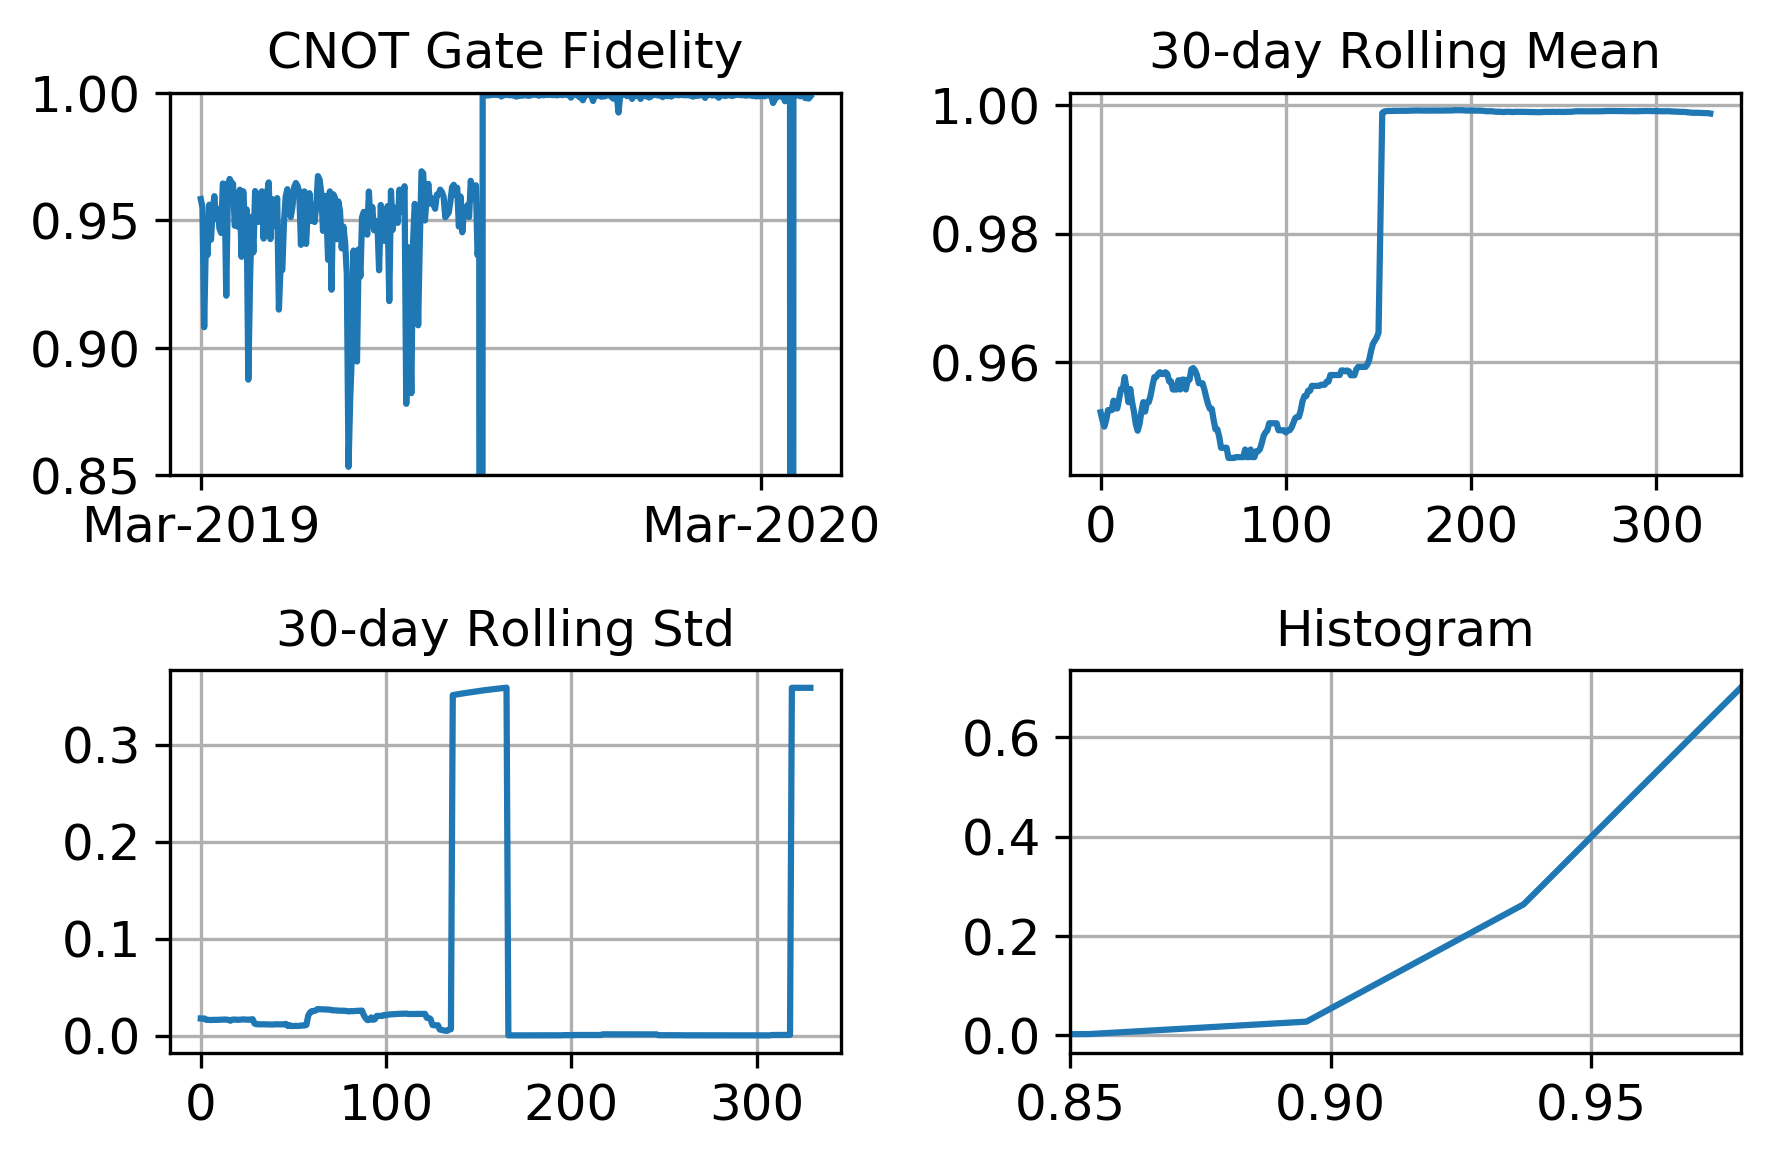
\includegraphics[width=6.6cm]{FG_stats.png}
\end{tabular}
& \begin{tabular}{l}
\scriptsize
\parbox{0.3\linewidth}{


\begin{itemize}
\item The plots show (in clockwise order): (a) time-series,\\ (b) the 30-day rolling mean,\\ (c) the histogram, \\ (d) the 30-day rolling standard deviation.
\end{itemize}
}
\end{tabular}
\end{tabular}

\scriptsize
\begin{center}
\minibox[frame]{
The publicly-available data provided by IBM is processed `as-is' and we defer efforts to \\validate the experimental data collection process itself.}
\end{center}
\end{frame}

%%%%%%%%%%%%%%%%%%%%%%%
\begin{frame}
\frametitle{Part II: The concept of temporal stability\\ \small{Using CNOT Gate Fidelity (referenced to March 2019 data)}}
\begin{textblock*}{50mm}(118mm,1mm)
\scriptsize
\textcolor{white}{\textbf{IEEE}}
\end{textblock*}
\begin{textblock*}{100mm}(5mm,92mm)
\scriptsize
\textcolor{white}{SOURCE: arXiv: 2008.09612}
\end{textblock*}
\vspace{0.1in}

\begin{tabular}{cl}  
\begin{tabular}{c}
%\includegraphics[width=6.6cm]{gate_err_control_chart.png}
\end{tabular}
& \begin{tabular}{l}
\scriptsize
\parbox{0.33\linewidth}{


\begin{itemize}
\item Data from Mar-2019 serves as the reference distribution.
\item Subsequent points measure the distance between the reference distribution and the distribution observed in a specific month.
\item The sharp improvement in gate fidelity around September 2019 corresponded to changes in hardware.
\end{itemize}
}
\end{tabular}
\end{tabular}

%\scriptsize
%\begin{itemize}
%\item The sharp improvement in gate fidelity around September 2019 corresponded to changes in hardware.
%\end{itemize}

\end{frame}

%%%%%%%%%%%%%%%%%%%%%%%%%%
\begin{frame}
\frametitle{Part II: The concept of spatial stability\\ \small{Using CNOT Gate Fidelity referenced to (0,1) between Mar19 - Mar20}}
\begin{textblock*}{50mm}(118mm,1mm)
\scriptsize
\textcolor{white}{\textbf{IEEE}}
\end{textblock*}
\begin{textblock*}{100mm}(5mm,92mm)
\scriptsize
\textcolor{white}{SOURCE: arXiv: 2008.09612}
\end{textblock*}
\vspace{0.1in}

\begin{tabular}{cl}  
\begin{tabular}{c}
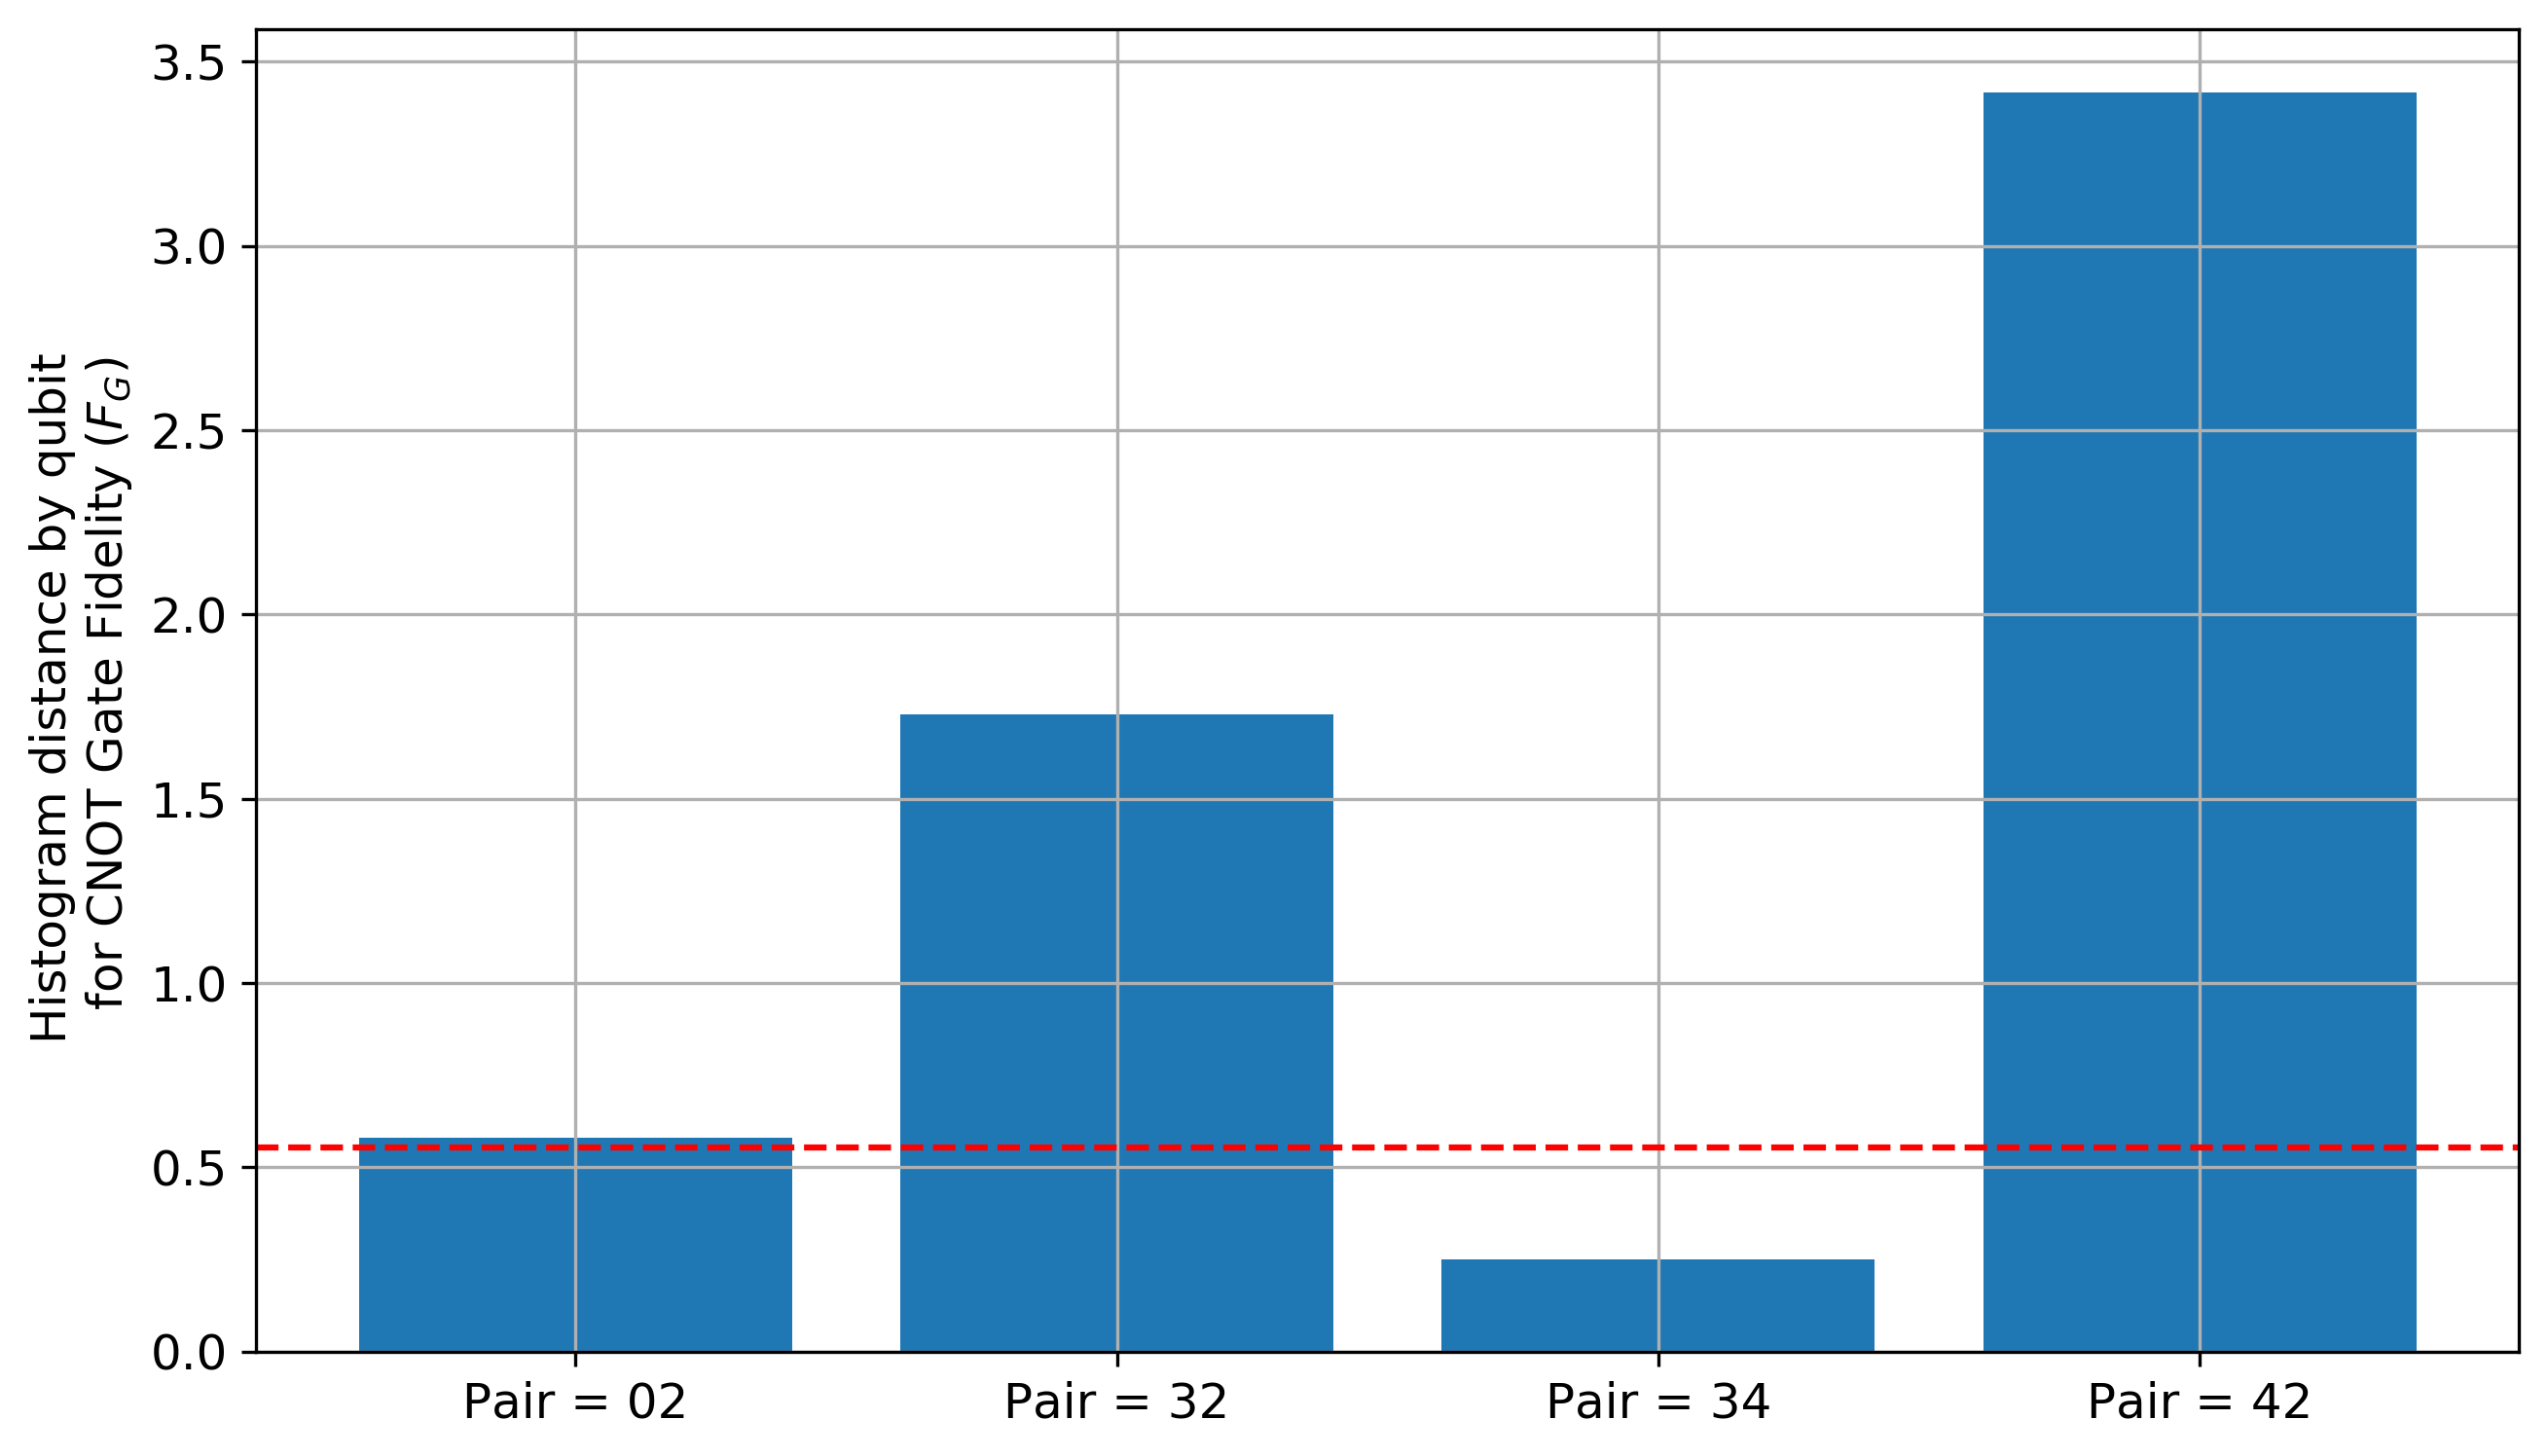
\includegraphics[width=6.6cm]{FG_spatialControlChart.png}
\end{tabular}
& \begin{tabular}{l}
\scriptsize
\parbox{0.3\linewidth}{


\begin{itemize}
\item Plot of the moment-based distance $d_4$ with respect to the physical layout.
\item Distance fluctuates spatially as well.
\end{itemize}
}
\end{tabular}
\end{tabular}

\scriptsize
\begin{center}

\textcolor{blue}{Concluding thoughts}:
\begin{itemize}
\item \textcolor{blue}{How to decide the stability threshold?}
\item \textcolor{blue}{How should the threshold depend on the application?}
\item \textcolor{blue}{What is the best way to decide the reference distribution?}
\item \textcolor{blue}{How to generalize the MBD for multi-variate cases?}
\end{itemize}

\end{center}

\end{frame}

%%%%%%%%%%%%%%%%%%%%%%

\end{document}

